\subsection{Network architecture}
\label{subsec:architecture}


The \ac{ANN} has an input layer and a \pLayer{} \cite{SNN}.
The input layer consists of $28 x 28$ neurons, i.e. one for each input pixel.
All the neurons of the input layer are connected to all the neurons of the \pLayer{} (all-to-all).

The \pLayer{} has \eN{}s and \iN{}s.
While every \eN{} is connected to exactly one \iN{} (one-to-one), every \iN{} is connected to all \eN{}s except the one it is already connected to.
This structure creates lateral inhibition and creates competition among the \eN{}s.

\begin{figure}[htbp]
    \center
    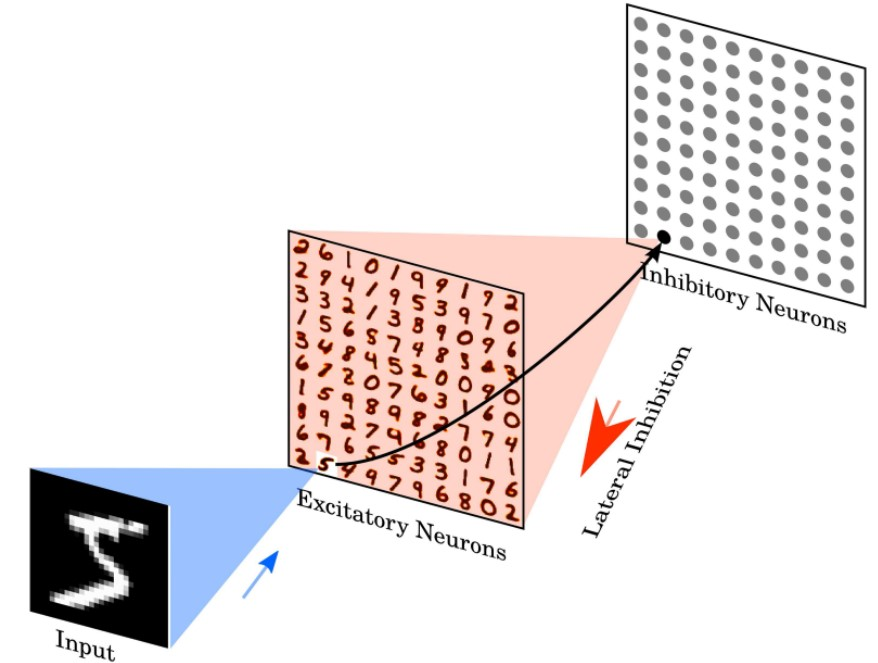
\includegraphics[width=0.5\textwidth]{pictures/architecture_SNN_erste_Quelle.jpg}
    \caption{architecture of the \ac{SNN} from \cite{SNN}}
    \label{fig:architecture_SNN}
\end{figure}